% Created 2024-05-18 Sat 17:06
% Intended LaTeX compiler: xelatex
\RequirePackage{fix-cm}
\PassOptionsToPackage{svgnames}{xcolor}
\documentclass[11pt]{article}
\usepackage{fontspec}
\usepackage{sectsty}
\allsectionsfont{\sffamily}
\usepackage{enumitem}
\setlist[description]{style=unboxed,font=\sffamily\bfseries}
\usepackage{listings}
\lstset{frame=single,aboveskip=1em,
	framesep=.5em,backgroundcolor=\color{AliceBlue},
	rulecolor=\color{LightSteelBlue},framerule=1pt}
\usepackage{xcolor}
\newcommand\basicdefault[1]{\scriptsize\color{Black}\ttfamily#1}
\lstset{basicstyle=\basicdefault{\spaceskip1em}}
\lstset{literate=
	    {§}{{\S}}1
	    {©}{{\raisebox{.125ex}{\copyright}\enspace}}1
	    {«}{{\guillemotleft}}1
	    {»}{{\guillemotright}}1
	    {Á}{{\'A}}1
	    {Ä}{{\"A}}1
	    {É}{{\'E}}1
	    {Í}{{\'I}}1
	    {Ó}{{\'O}}1
	    {Ö}{{\"O}}1
	    {Ú}{{\'U}}1
	    {Ü}{{\"U}}1
	    {ß}{{\ss}}2
	    {à}{{\`a}}1
	    {á}{{\'a}}1
	    {ä}{{\"a}}1
	    {é}{{\'e}}1
	    {í}{{\'i}}1
	    {ó}{{\'o}}1
	    {ö}{{\"o}}1
	    {ú}{{\'u}}1
	    {ü}{{\"u}}1
	    {¹}{{\textsuperscript1}}1
            {²}{{\textsuperscript2}}1
            {³}{{\textsuperscript3}}1
	    {ı}{{\i}}1
	    {—}{{---}}1
	    {’}{{'}}1
	    {…}{{\dots}}1
            {⮠}{{$\hookleftarrow$}}1
	    {␣}{{\textvisiblespace}}1,
	    keywordstyle=\color{DarkGreen}\bfseries,
	    identifierstyle=\color{DarkRed},
	    commentstyle=\color{Gray}\upshape,
	    stringstyle=\color{DarkBlue}\upshape,
	    emphstyle=\color{Chocolate}\upshape,
	    showstringspaces=false,
	    columns=fullflexible,
	    keepspaces=true}
\usepackage[a4paper,margin=1in,left=1.5in]{geometry}
\usepackage{parskip}
\makeatletter
\renewcommand{\maketitle}{%
  \begingroup\parindent0pt
  \sffamily
  \Huge{\bfseries\@title}\par\bigskip
  \LARGE{\bfseries\@author}\par\medskip
  \normalsize\@date\par\bigskip
  \endgroup\@afterindentfalse\@afterheading}
\makeatother
\usepackage{graphicx}
\usepackage{grffile}
\usepackage{longtable}
\usepackage{wrapfig}
\usepackage{rotating}
\usepackage[normalem]{ulem}
\usepackage{amsmath}
\usepackage{textcomp}
\usepackage{amssymb}
\usepackage{capt-of}
\usepackage{hyperref}
\hypersetup{linkcolor=Blue,urlcolor=DarkBlue,
  citecolor=DarkRed,colorlinks=true}
\AtBeginDocument{\renewcommand{\UrlFont}{\ttfamily}}
\author{Bruno Alves}
\date{\today}
\title{}
\hypersetup{
 pdfauthor={Bruno Alves},
 pdftitle={},
 pdfkeywords={},
 pdfsubject={},
 pdfcreator={Emacs 30.0.50 (Org mode 9.6.15)}, 
 pdflang={English}}
\begin{document}

\tableofcontents

The CMS experiment adopts a right-handed coordinate system, with the origin placed at the nominal collision point.
The x-axis points toward the centre of the LHC ring, the y-axis points vertically upward, and the z-axis thus points towards the Jura mountains.
The structure of the detector makes it natural to use a polar coordinate system.
The azimuthal angle \(\phi\) is measured in the \(x - y\) plane from the x-axis, the radial coordinate is given by \(r\), and the polar angle \(\theta\) is measured from the z-axis in the \(y - z\) plane.
A schematic representation of the CMS coordinate system is shown in Fig. 2.5.
The relation between the Cartesian and the CMS coordinates is given by:

\begin{equation}
\label{eq:orga8160aa}
\begin{cases}
x = r \sin \theta \cos \phi \\
y = r \sin \theta \sin \phi \\
z = r \cos \theta
\end{cases}
\end{equation}

While this coordinate system is well suited for expressing the orientation of the detector and macroscopic observables, it is not ideal for describing proton-proton collisions.
A proton-proton collision is actually a parton-parton collision.
Protons, not being fundamental particles, are made of different constituents, named partons.
Consider a scenario where two protons collide head-on.
The four-momentum of the two partons can be written as:

\begin{equation}
\label{eq:org4f913d5}
\begin{cases}
p^{\mu}_1 = (x_1E, 0, 0, x_1p) \\
p^{\mu}_2 = (x_2E, 0, 0, -x_2p) \\
\end{cases}
\end{equation}

In these four-vectors, \(E\) and \(p\) denote the energy and momentum of the proton, respectively.
The \(x\) and \(y\) components are null as protons are primarily accelerated longitudinally at high energies, leading to negligible transverse momentum for the partons inside them.
Consequently, the \(x_1\) and \(x_2\) variables can be interpreted as the fractions of energy that the partons carry away from the original protons.
After the collision, the resulting momentum is given by:

\begin{equation}
\label{eq:orgfcf9e2c}
(p_1 + p_2)^{\mu} = ((x_1 + x_2)E, 0, 0, (x_1 - x_2)p)
\end{equation}

The CMS frame is not the centre-of-mass frame of the collision.
The relativistic \(\beta\) factor, in the high-energy limit where \(E \approx p\), results to be:

\begin{equation}
\label{eq:orgeec9278}
\beta = \frac{x_1 - x_2}{x_1 + x_2}
\end{equation}

The \(x_1\) and \(x_2\) quantities are unknown and change from event to event, consequently also the related Lorentz-boost is unknown.
It is thus beneficial to use variables that are Lorentz-invariant for boosts along the longitudinal direction.
The par excellence observables are the transverse momentum \(p_T\) and transverse mass \(m_T\):

\begin{equation}
\label{eq:orgecb361f}
\begin{cases}
p^2_T = p^2_x + p^2_y \\
m^2_T = m^2 + p^2_x + p^2_y = E^2 - p^2_z \\
\end{cases}
\end{equation}


From these variables, the transverse energy is defined as:
\begin{equation}
\label{eq:org0a02e39}
E^2_T = m^2 + p^2_T
\end{equation}

which is equal to the transverse momentum for massless particles.
Another variable is the rapidity \(y\):

\begin{equation}
\label{eq:orgc2903b7}
y = \frac{1}{2} \ln \left( \frac{E + p_z}{E - p_z} \right)
\end{equation}

A Lorentz-boost along the z-axis shifts the rapidity by a constant term that depends on the boost itself.
The rapidity itself is thus not Lorentz-invariant; its difference is.
One of the advantages of using the rapidity is that particle production is roughly constant as a function of \(y\).
For ultra-relativistic particles, the rapidity is usually converted to the pseudorapidity \(\eta\):


\begin{equation}
\label{eq:org9cc3992}
y \approx \frac{1}{2} \ln \left( \frac{E(1 + \cos \theta)}{E(1 - \cos \theta)} \right)
= -\frac{1}{2} \ln \left( \tan \left( \frac{\theta}{2} \right) \right)
\equiv \eta
\end{equation}

The pseudorapidity is a pure geometrical variable, depending only on the angle \(\theta\).
It can be also used to define a Lorentz-invariant spatial separation between two particles:

\begin{equation}
\label{eq:org1563540}
\Delta R = \sqrt{(\Delta \eta)^2 + (\Delta \phi)^2}
\end{equation}

Based on the \(\eta\) coordinate, the detector is divided into a central part called barrel, and two forward parts called endcaps.
The exact \(\eta\) value marking the transition between the two regions depends on the specific sub-detector.

\begin{figure}
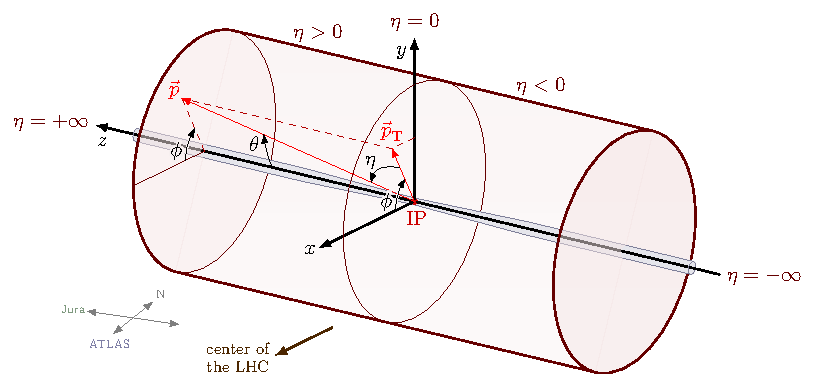
\includegraphics[width=1.\textwidth]{/home/bruno/org/PhD/Thesis/figures/detector/coordinates_left.pdf}
\caption{\label{orga184625}Coordinate system of the CMS detector. Courtesy of Izaak Neutelings \cite{izaak_neutelings}.}
\end{figure}
\end{document}
